% 00-page-de-titre.tex — Page de titre (compléter les champs entre crochets).

\begin{titlepage}
  \centering
  \vspace*{1cm}
  {\large\textsc{[Université]} \par}
  \vspace{0.2cm}
  {\large [Faculté — programme de master] \par}
  \vspace{2.5cm}
  {\color{accent}\rule{\linewidth}{1.2pt}\par}
  \vspace{0.6cm}
  {\Huge\bfseries Des simulations interactives pour enseigner la mécanique en première année d'ingénieur civil \par}
  \vspace{0.4cm}
  {\Large Conception assistée par IA, ludification et évaluation \par}
  \vspace{0.6cm}
  {\color{accent}\rule{\linewidth}{1.2pt}\par}
  \vspace{1.5cm}
  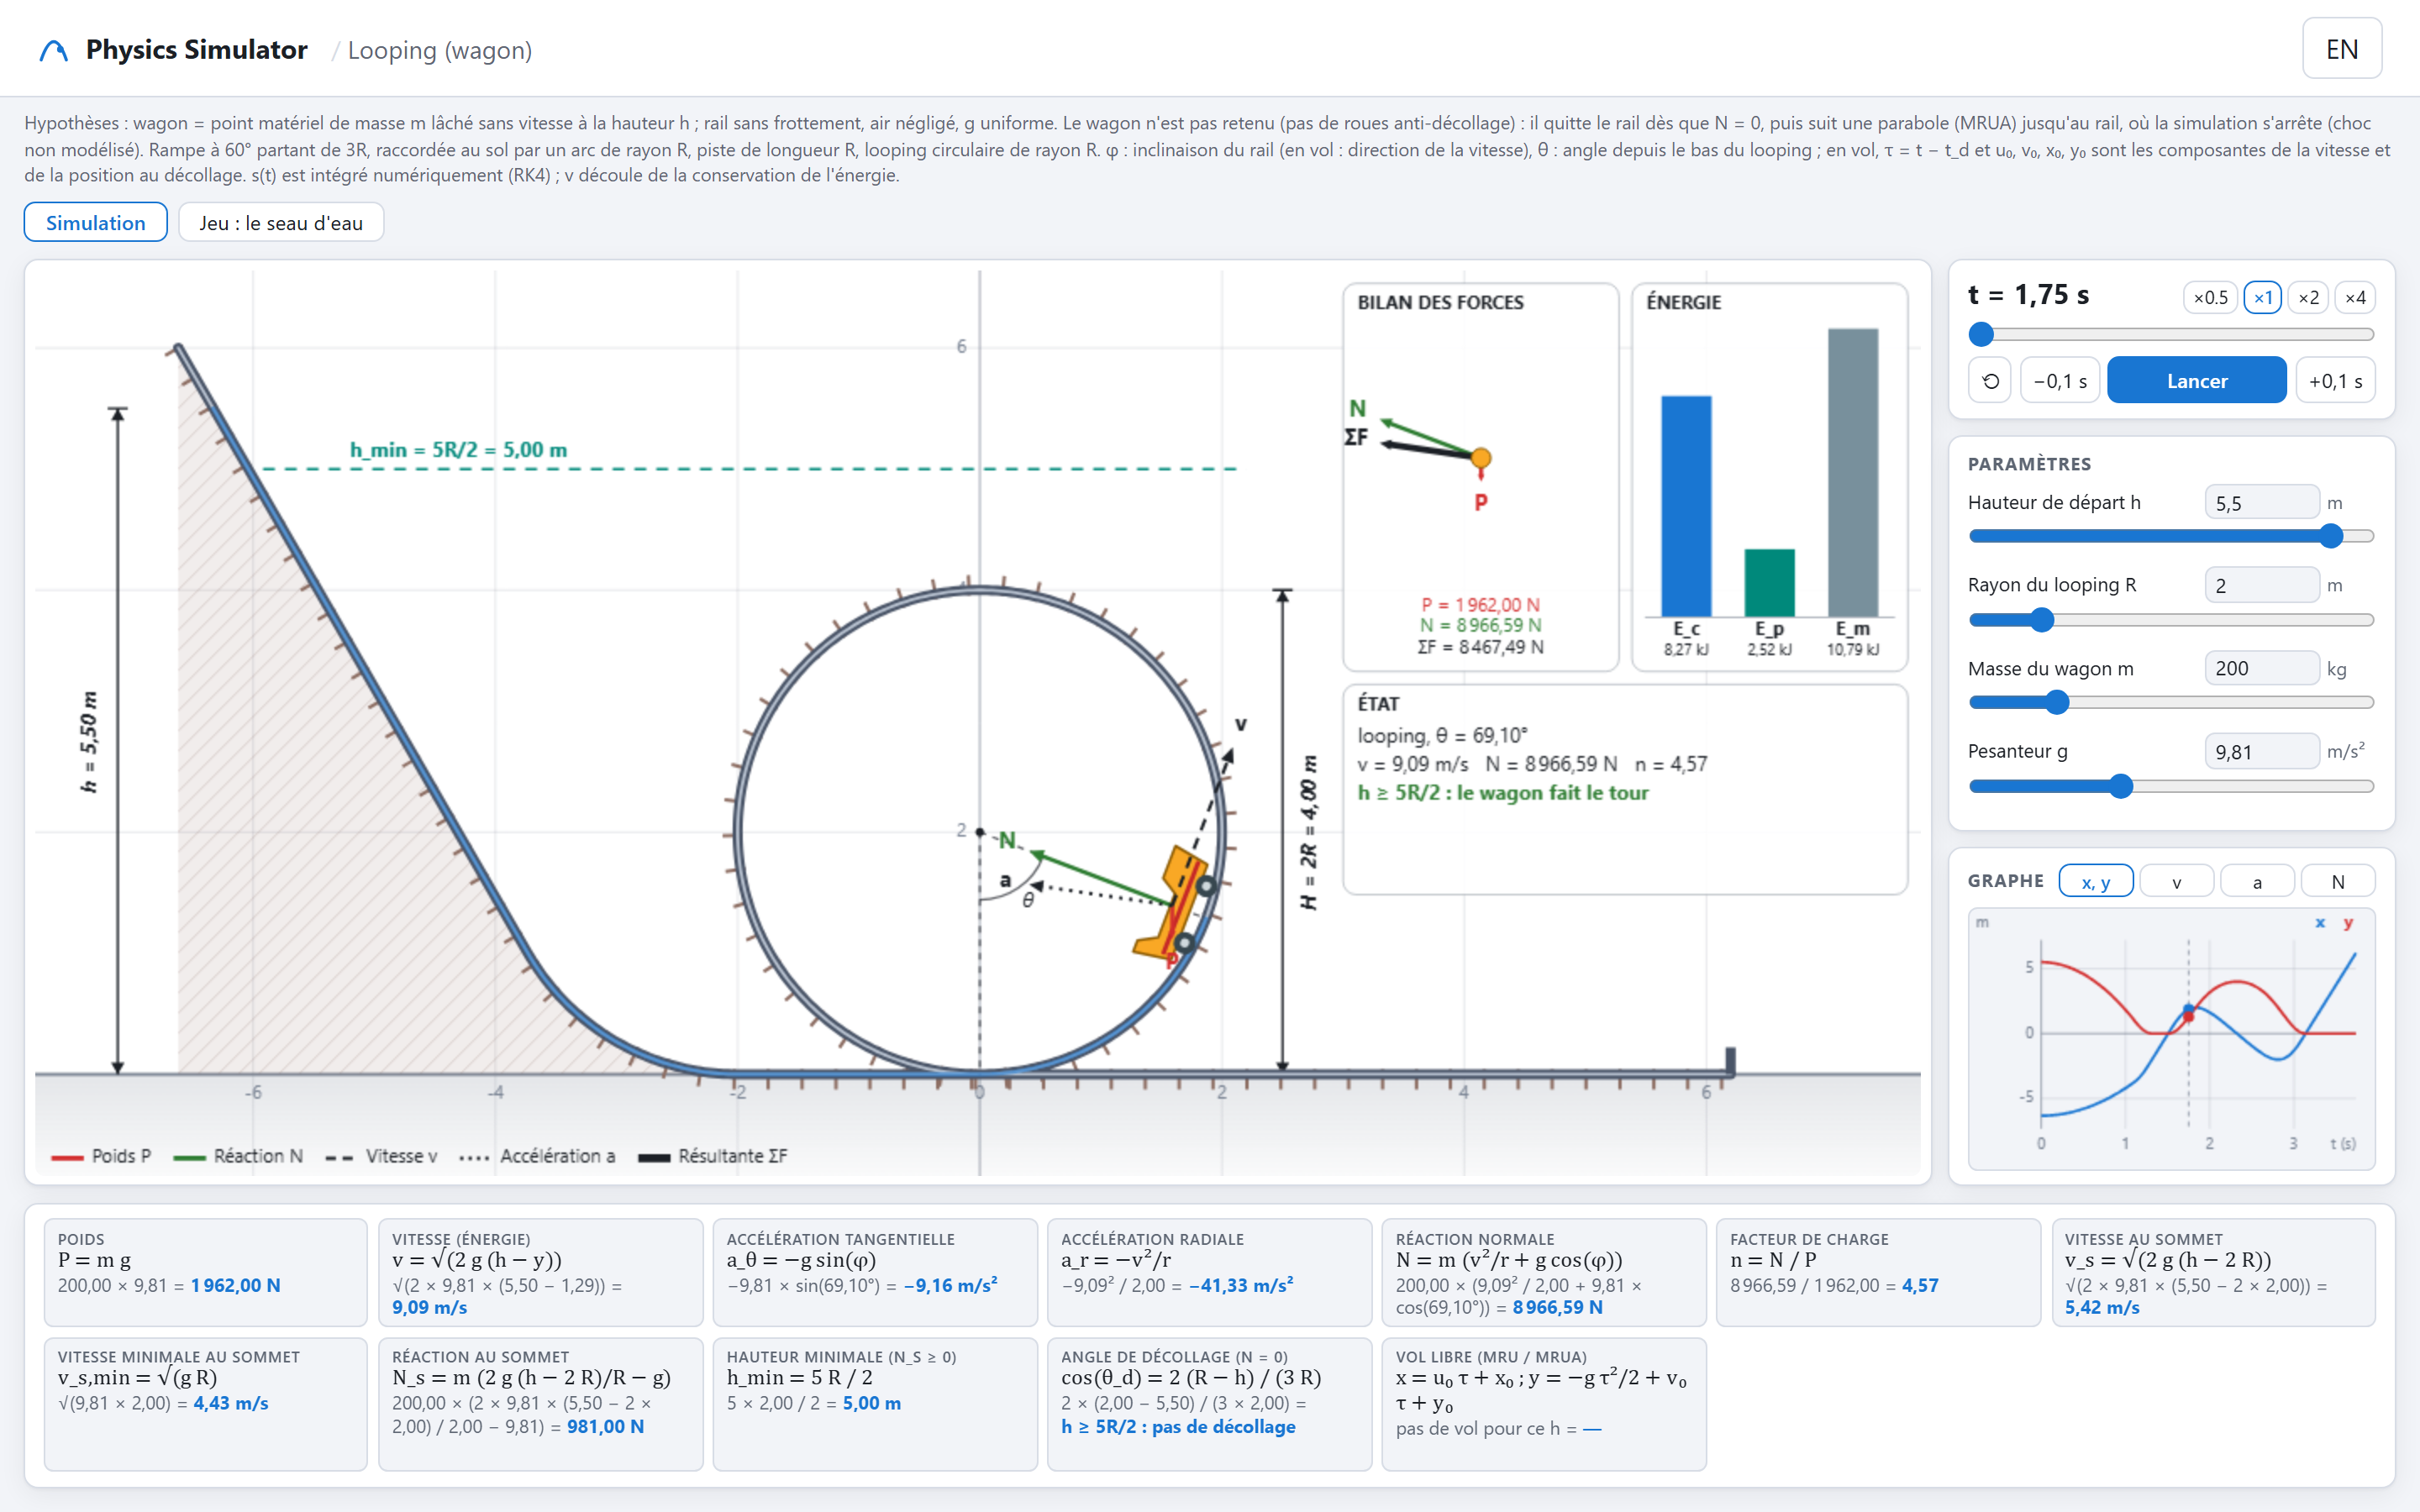
\includegraphics[width=0.78\linewidth]{figures/captures/looping-ecran-complet.png}
  \vfill
  \begin{tabular}{@{}ll@{}}
    Auteur : & Arnaud Gheysens \\
    Promoteur : & [Nom du promoteur] \\
    Lecteurs : & [Noms des lecteurs] \\
  \end{tabular}
  \par\vspace{1cm}
  {\large Mémoire présenté en vue de l'obtention du grade de [master] \par}
  {\large Année académique [2026--2027] \par}
\end{titlepage}
